%----------------------------------------------------------------------------
\chapter{Technológiák}\label{sect:technologia}
%----------------------------------------------------------------------------

Diplomatervem készítése során többféle szoftveres és hardveres technológiával kellett megismerkednem. Jelen fejezet megírásával az a célom, hogy az olvasó képet kapjon a felhasznált szoftver- és hardvereszközök fejlődéséről, valamint jelenlegi állapotukról; együttesen hogy megindokoljam, miért ezeket a technológiákat választottam a dolgozatom témáját feldolgozó alkalmazás megírásakor.

\bigskip

A fejezet \sectref{opencv} szakaszában az OpenCV gépi látás könyvtár, a \sectref{qt} szakaszában pedig a Qt keretrendszer rövid, összefoglaló jellegű bemutatására vállalkozom. A fejezet utolsó harmadában a projekthez felhasznált webkamera kiválasztását, összeállítását, illetve előnyeit/hátrányait dokumentálom. 

%,,,,,,,,,,,,,,,,,,,,,,,,,,,,,,,,,,,,,,,,,,,,,,,,,,,,,,,,,,,,,,,,,,,,,,,,,,,,
\section{Az OpenCV könyvtár}\label{sect:opencv}
%,,,,,,,,,,,,,,,,,,,,,,,,,,,,,,,,,,,,,,,,,,,,,,,,,,,,,,,,,,,,,,,,,,,,,,,,,,,,

\begin{wrapfigure}{r}{0.3\textwidth}
  \begin{center}
    
\includegraphics[width=0.28\textwidth]{figures/opencv_logo.png}
  \end{center}
\end{wrapfigure}

Az \textbf{OpenCV}\footnote{\url{http://opencv.org/}} egy nyílt forráskódú gépi látás (computer vision) könyvtár. Elsődleges célja, keretet nyújtani \textbf{valósidejű} képfeldolgozási alkalmazások fejlesztésére. A könyvtár szabadon letölthető és felhasználható a BSD licenc\footnote{\url{http://www.linfo.org/bsdlicense.html}} keretein belül. \cite{opencv_wiki}

\bigskip

Az OpenCV projekt hivatalosan 1999-ben indult az Intel kezdeményezésében. A nagyközönségnek a 2000. évi \textit{,,IEEE Conference on Computer Vision and Pattern Recognition''} konferencián mutatkozott be, majd öt béta-verziót követően 2006-ban jutott el az 1.0-ás hivatalos kiadásig. A fejlesztése itt úgy tűnt, hogy megáll, de végül a projektet a Willow Garage\footnote{\url{http://www.willowgarage.com/}} robotikai kutatólabor vette szárnyai alá. Az ő irányításuk alatt 2008 októberében elkészült az 1.1-es verzióval közel egy időben látott napvilágot az elsõ hivatalos OpenCV-vel foglalkozó könyv \textit{,,Learning OpenCV: Computer Vision with the OpenCV Library''} címmel Gary Bradski és Adrian Kaehler fejlesztők tollából \cite{opencv_book}. Az egy évvel később, 2009 októberében megjelent 2.0-ás verzióval a projekt nagy fejlődésen esett át. Ebben a verzióban található meg először a C++ és Python interfész (ez a meglévő C mellett már három hivatalosan fejlesztett interfészt jelentett), amely az egyszerűbb kezelhetőség, új függvények mellett a meglévő eljárások teljesítmény tekintetében -- különösen többmagos rendszereken -- jobb implementációját kínálta a felhasználóknak.

\bigskip

A projekt életében a következő mérföldkő 2012 augusztusa volt. Ekkor az OpenCV támogatását és fejlesztését az erre a célra alapított \emph{OpenCV.org} non-profit alapítvány vette át. A 2.5-ös verzió kiadásával tovább bővült a támogatott programozási nyelvek listája: innentől már a Java és a MATLAB/OCTAVE is felkerült az elérhető interfészek listájára. Nem hivatalos támogatással, de további wrapper-ek is elérhetők a könyvtárhoz, például C\# vagy Ruby nyelven, ezzel is elősegítve a széleskörű elterjedését. 

Az elmúlt években a GPU-gyorsítás támogatása terén is komoly előrelépésekre került sor. 2010 szeptemberétől érhető el a CUDA, 2012 októberétől pedig az OpenCL interfész.

\bigskip

A fejlesztést különböző platformokra párhuzamosan (\textbf{cross-platform}) történik. Mivel a könyvtár alapvetően a C nyelvre épül, ezért a számos rendszeren működésre bírható. A dolgozat írásának idején elérhető 2.5-ös stabil verzió a következő operációs rendszerekre elérhető:

\begin{itemize}
  \item asztali (desktop) rendszerek
  \begin{itemize}
    \item Windows
    \item Linux
    \item OS X
    \item OpenBSD
    \item FreeBSD  
  \end{itemize}
  \item mobil operációs rendszerek
  \begin{itemize}
    \item iOS
    \item Android
    \item BlackBerry 10
    \item Maemo
  \end{itemize}   
\end{itemize}

Az OpenCV jelenleg elérhető 2.5-ös verziója széles körben, mondhatni világszerte használt, felhasználói tábora több, mint 47\,000 főt számlál. Köszönhető ez többek között annak, hogy felhasználási lehetőségei igencsak sokrétűek: több, mint 500 optimalizált algoritmust kínál annak érdekében, hogy ,,ne kelljen újra feltalálnunk a kereket''. Sebesség tekintetében érződik a kipróbált, optimalizált algoritmusok használata: az OpenCV a jelenleg elérhető leggyorsabb alternatíva gépi látás terén (\figref{opencv_speed} ábra). Teljesítménye azonban adott esetben még tovább növelhető, mivel ha Intel IPP\footnote{\url{http://software.intel.com/en-us/intel-ipp/}} (Integrated Performance Primitives) támogatást észlel, az abban található szálakra optimalizált algoritmusok használatát fogja preferálni.

\begin{figure}[!ht]
\centering
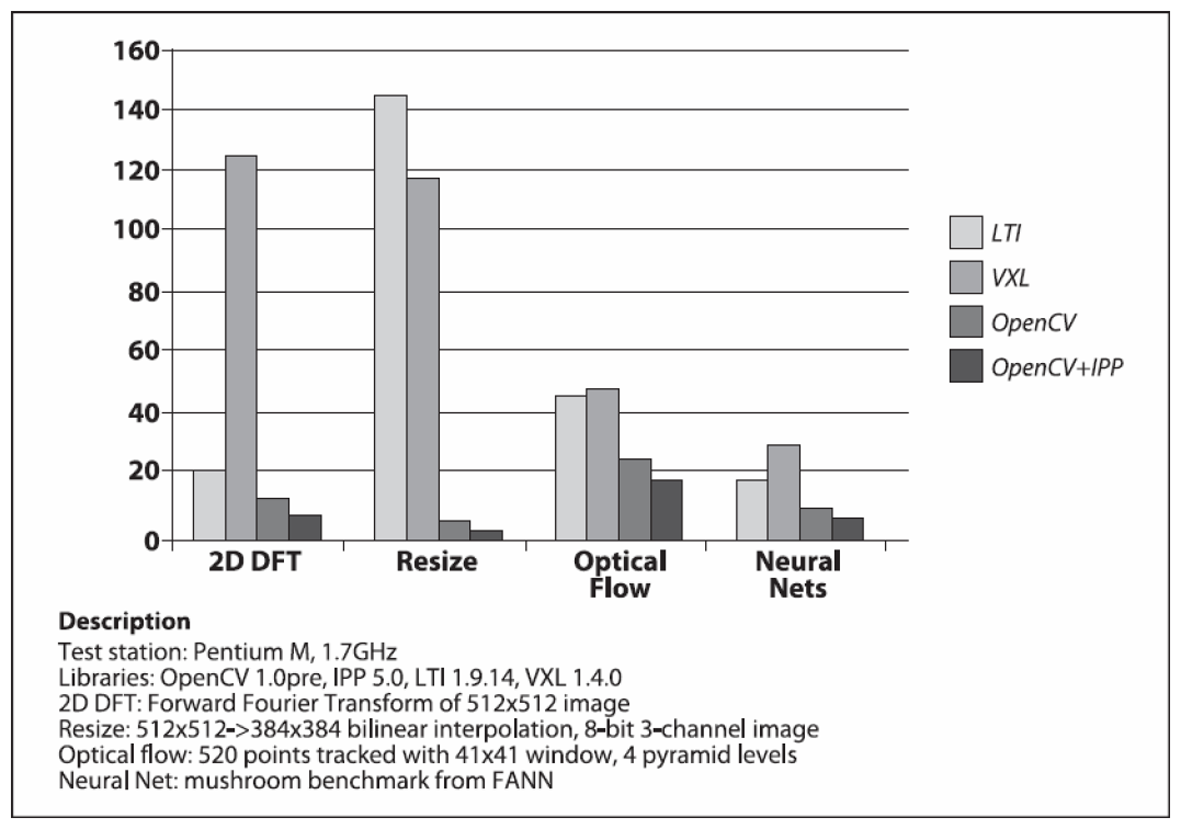
\includegraphics[width=100mm, keepaspectratio]{figures/opencv_speed.png}
\caption{Az OpenCV teljesítménye az LTI és VXL képfeldolgozási könyvtárakkal összehasonlítva.\\Forrás: \cite{opencv_book}}
\label{fig:opencv_speed}
\end{figure}

A teljes funkcionalitás részletekbe menő bemutatása -- mint láthattuk \cite{opencv_book} -- egy könyvet is megtölt, de a teljesség igénye nélkül tekintsük át, hogy milyen alapvető jellemzői és alkalmazásai vannak a környezetnek:

\begin{itemize}

 \item alap adatstruktúrák
  \begin{itemize}
   \item mátrixok, vektorok
  \end{itemize} 

 \item mátrix és vektor manipuláció, lineáris algebra
  
 \item dinamikus adatstruktúrák
  \begin{itemize}
   \item listák, sorok, halmazok
   \item gráfok és fák
  \end{itemize}

 \item kép és videó input/output
  \begin{itemize}
   \item beolvasás fájlból (kép vagy videó) és kameráról
   \item kiírási lehetőség képként vagy videóként
  \end{itemize}

 \item előfeldolgozás
  \begin{itemize}
   \item él- és sarokkeresés
   \item mintavételezés és interpoláció
   \item színkonverzió
   \item morfológiai operátorok
  \end{itemize}

 \item struktúraanalízis
  \begin{itemize}
   \item távolság- és Hough-transzformáció
   \item kontúrfeldolgozás
   \item sablonillesztés
   \item különböző momentumok
   \item Delaunay háromszögelés
  \end{itemize}

 \item kamerakalibráció
  \begin{itemize}
   \item kalibrációs mintázatok felismerése és követése
   \item fundamentális mátrix becslés
   \item homográfia becslés
   \item sztereó megfeleltetés
  \end{itemize}
  
 \item mozgásanalízis
  \begin{itemize}
   \item optical flow
   \item mozgásszegmentálás és -követés
  \end{itemize}

 \item objektumfelismerés
  \begin{itemize}
   \item eigen-módszerek
   \item rejtett Markov-modell (Hidden Markov Model -- HMM)
  \end{itemize}
  
  \item kiterjesztett valóság-támogatás (Augmented Reality -- AR)
  
  \item gépi tanulás könyvtár
  \begin{itemize}
    \item döntési fa-alapú tanulás
    \item klaszterezési algoritmusok (pl. k-szomszédság)
    \item neurális hálózatok
    \item Bayes-osztályozó
    \item szupport vektor gépek (Support Vector Machine -- SVM)
  \end{itemize}    
  
 \item GUI és rajzolás
  \begin{itemize}
   \item kép és videó megjelenítés
   \item billentyűzet és egérkezelés
   \item egyenes, kör, poligon, szöveg rajzolása
  \end{itemize}
  
\end{itemize}

Láthatjuk, hogy a fent felsorolt funkciókkal a gépi látás terén rengeteg egyszerűbb feladatot szinte ,,egy lépésben'', beépített, optimalizált eljárások segítségével oldhatunk meg. Ha nagyobb szabású projektbe kezdünk, akkor is hasznunkra lehet, hogy részben vagy egészében egy több tízezres felhasználói tábor (melynek jelentős részét aktív kutatók alkotják) visszajelzései alapján fejlesztett környezetre építhetjük munkánkat.

\bigskip

Az OpenCV régebbi verzióiban a számos előny mellett hátrányként volt megemlíthető, hogy segítségével a felhasználói felületet csak nagyon leegyszerűsített módon szabhattuk testre. Igaz, hogy a könyvtár feladata elsősorban a képfeldolgozás és nem a megjelenítés, így ebből a nézőpontból a beépített kép és videó megjelenítési lehetőség, billentyűzet- és egérkezelés valamint trackbarok (csúsztatható kezelőszerv értékek beállítására) létrehozásának lehetősége inkább hozzáadott értékként jelent meg, azonban ez nem változtat azon a tényen, hogy ha igény van felhasználóbarát kezelőfelület készítésére, az OpenCV-t mindenképpen integrálnunk kellett valamely elterjedt grafikus felhasználói felület toolkittel.

A 2.1-es verziótól kezdődően megjelent egy némileg fejlettebb \textbf{Qt alapú felhasználói felület}. Teljes szabadságot még ez sem ad a felületek kialakításában, de az egyszerűbb projektek kezelőszerveinek és megjelenítésének problémája már kielégítően elvégezhető egyéb eszköz használata nélkül.

%,,,,,,,,,,,,,,,,,,,,,,,,,,,,,,,,,,,,,,,,,,,,,,,,,,,,,,,,,,,,,,,,,,,,,,,,,,,,
\section{A Qt keretrendszer}\label{sect:qt}
%,,,,,,,,,,,,,,,,,,,,,,,,,,,,,,,,,,,,,,,,,,,,,,,,,,,,,,,,,,,,,,,,,,,,,,,,,,,,

A \textbf{Qt}\footnote{\url{http://qt.digia.com/}} (ejtsd az angol ,,cute'' szó mintájára: kjút) keretrendszer egy széles körben használt szoftver, amelyet egyrészt grafikus felhasználói felületek (Graphical User Interface -- GUI), másrészt parancssoros (Command Line Interface -- CLI) alkalmazások fejlesztésére is használnak. A grafikus felhasználói felületek fejlesztése során a Qt úgynevezett wiget-toolkitként funkcionál -- kis, önálló elemek (widgetek) felhasználását és összekötését teszi lehetővé, ezek összességéből áll össze az elkészült grafikus felület. A szoftver a  GPL~v3\footnote{\url{http://www.gnu.org/licenses/gpl.html}} illetve LGPL~v2\footnote{\url{http://www.gnu.org/licenses/lgpl-2.1.html}} licencek szerint szabadon elérhető. \cite{qt_wiki}

A keretrendszer egyik nagy előnyének számít más rendszerekkel összehasonlítva, hogy a grafikus felületek kirajzolásakor minden operációs rendszeren igyekszik az elérhető natív elemeket használni, ennek köszönhetően (a natív kirajzolásokból származó nagyszerű performancia mellett) a Qt-tal fejlesztett alkalmazások semelyik platformon nem tűnnek rendszeridegennek.

\bigskip

A Qt projekt első hivatalos kiadása a Nokia \emph{Qt Development Frameworks} csoport égisze alatt látta meg a napvilágot, miután a finn mobilgyártó felvásárolta a technológiát a norvég Trolltech vállalattól. Ennek megfelelően a kezdeti években az asztali platformok mellett leginkább a Symbian operációs rendszer támogatása jelentette a fő csapásirányt. A Nokia azonban 2011-ben szakított saját fejlesztésű operációs rendszerével, és a további bizalmát a Microsoft akkori és elkövetkező mobilplatformjaiba (Windows Phone~7, majd 8) fektette.

Ezt követően a Nokia megvált a rendszer kereskedelmi jogaitól, és azok a Digia\footnote{\url{http://www.digia.com/}} vállalathoz kerültek, amely azóta is a projekt karbantartója, bár a tényleges fejlesztői munka nagy részét továbbra is a Nokia mérnökei végzik. A tranzakció után az új tulajdonos közvetlen célnak tűzte ki, hogy aktualizálják a Qt által támogatott platformok listáját az időközben népszerűvé vált rendszerekkel.

A dolgozat írásakor támogatott fontosabb operációs rendszerek:

\begin{itemize}
  \item Windows (XP és 7)
  \item OS X
  \item Linux, FreeBSD, OpenBSD
  \item iOS
  \item Android
  \item QNX (BlackBerry 10)
\end{itemize}

A Qt-ot használó alkalmazások programozási nyelve alapvetően a sztenderd C++, a \emph{Meta Object Compiler} (moc) kódgenerátorral kiegészítve, amely számos beépített makróval teszi könnyebbé a fejlesztést. Több más programozási nyelv is használható az ún. \textbf{kötések} (bindings) használatával. A Qt~4-es verziójához elérhető kötések listája a teljesség igénye nélkül:

\begin{itemize}
  \item C\# és .NET
  \item Java
  \item Python
  \item szkriptnyelvek
  \begin{itemize}
    \item Perl
    \item Ruby
    \item PHP
    \item Tcl
  \end{itemize}    
   
\end{itemize}

A Qt a GUI események célba juttatását a \textbf{signals/slots} rendszer segítségével végzi. A módszer az \emph{Observer}\footnote{\url{http://en.wikipedia.org/wiki/Observer_pattern}} (Megfigyelő) tervezési minta megvalósítására nyújt egyszerű és szabványosított lehetőséget. A felhasználói felület elemei (widgetek) jelzéseket (signal) bocsátanak ki -- pl. ,,a X gombot megnyomták'', ,,a beviteli mező értéke Y-ra változott'' -- amelyeket más elemek ,,foglalataihoz'' (slot) köthetünk, ahol az eseményt lekezelhetjük. Látható, hogy ez a struktúra remekül illeszkedik a grafikus felhasználói felülete eseménykezelésére, de ezen kívül időzítések és értesítések kézbesítésére is alkalmas.

A signalok és slotok a megvalósításukat tekintve speciális  függvények, melyeket deklarálásukkor a két bekezdéssel előbb említett \emph{moc} (Meta Object Compiler) automatikusan generál, elkerülve ezzel a feleslegesen ismétlődő kódrészletek elburjánzását (boilerplate kód).

\bigskip

A Qt~4-es verziójához nagyjából 6 éven át érkeztek a kisebb/nagyobb frissítések, egészen a 4.8-as kiadásig. Ezt követően a koncepcionális változásokat hozó \textbf{Qt 5} fejlesztése folytatódik tovább. Az 5-ös verzió funkciói között között a hardveres gyorsítású megjelenítés, a QML\footnote{\url{http://en.wikipedia.org/wiki/QML}} és a JavaScript támogatása jelentik a legfontosabb újdonságokat.

A Qt~5 kiadásával a keretrendszer tett egy lépést a nyílt (open source) fejlesztés irányába: a \textbf{Qt~Project}\footnote{\url{http://qt-project.org/}} néven futó projektbe már külsős fejlesztők is delegálhatják javításaikat vagy új funkciókat, amelyeket a Digia és a Nokia csapata elbírál, és ha megfelelőnek találtatnak, bekerülhetnek a soron következő verzióba.

%............................................................................
\subsection{A Qt Creator fejlesztői környezet}\label{sect:qt_creator}
%............................................................................

A \textbf{Qt Creator} egy integrált fejlesztői környezet (Integreated Development Environment -- IDE) Qt alapú fejlesztésekhez. Használatával jelentősen megkönnyíthető mind a grafikus felületek kialakítása, mind az alkalmazások forráskódjának szerkesztése és fordítása. \cite{qtcreator_wiki}

\paragraph{Szerkesztő}

A kódszerkesztő (editor) a kor követelményeinek megfelelően támogatja a szintaxis-kiemelést valamint az automatikus kódkiegészítést (code completion) több programozási nyelvre is. A szerkesztő hátrányának róható fel, hogy a megnyitott fájlokat nem a manapság elterjedt fülek (tab) használatával rendezi, hanem saját fejlesztésű listát használ erre a célra, amely más fejlesztői környezetekből érkezve kissé idegen.

\paragraph{Qt Designer}

A felhasználó felületek kialakításában nélkülözhetetlen segítséget nyújt a beépített Qt Designer eszköz. Használatával WYSIWYG (What You See Is What You Get) módon végezhetjük az alkalmazás grafikus felületének kialakítását. Választhatunk a számtalan beépített widget közül, de saját elemek létrehozását is támogatja a rendszer -- a widgetek fejlesztési konvencióit betartva az egyedi elemek is grafikusan jelennek meg a szerkesztőfelületen.

A felületek integrálása a kóddal az \sectref{qt} szakaszban említett signal-slot mechanizmus segítségével történhet, amelynek megvalósítása szintén nagyon felhasználóbarát módon sikerült.

\paragraph{Qt Quick Designer}

Ez az eszköz animációk fejlesztésére szolgál, amelyeket QML\footnote{\url{http://en.wikipedia.org/wiki/QML}} nyelvű leírásukkal adhatunk meg. A Qt natívan támogatja a nagyfrekvenciás (60 FPS) animációk készítését és lejátszását, ezáltal a 2D vagy 3D animációk ,,simák'', akadás mentesek lehetnek.

\paragraph{Verziókezelő-integráció}

A fejlesztői környezet képes a legnépszerűbb verziókezelő rendszerek támogatására. A támogatott rendszerek között van a népszerű \emph{Git} valamint \emph{Subversion (SVN)}, de \emph{CVS}, \emph{Bazaar} vagy \emph{Mercurial} kódbázisunkat is kezelhetjük közvetlenül a Qt Creatorral.

\paragraph{Példakódok}

Az alkalmazás nyitóképernyőjén rögtön számtalan példaprogram fogadja a felhasználót. A példák százas nagyságrendben érhetők el, és a legegyszerűbb feladatoktól (,,Hello World'') az egészen összetettekig próbálják lefedni a fejlesztés során esetlegesen felmerülő problémákat.

Letöltésük nem igényel többet néhány kattintásnál, és integrált megoldás lévén a kód betöltődik a szerkesztőbe -- azonnal futtathatjuk és elkezdhetjük megérteni a működését. Maga az ötlet, és a megvalósítás is példaértékű lehet más fejlesztőkörnyezetek számára, igazi kincsesbányát jelent a Qt működésében elmélyedni kívánó fejlesztők számára.

%,,,,,,,,,,,,,,,,,,,,,,,,,,,,,,,,,,,,,,,,,,,,,,,,,,,,,,,,,,,,,,,,,,,,,,,,,,,,
\section{Fejkamera}\label{sect:infracam}
%,,,,,,,,,,,,,,,,,,,,,,,,,,,,,,,,,,,,,,,,,,,,,,,,,,,,,,,,,,,,,,,,,,,,,,,,,,,,

A tekintetkövető rendszer fejlesztése közben hardveres technológiai kérdések is felmerültek. A legfontosabb ilyen kérdés a pupillát követő kamera kiválasztása és elhelyezése volt.

%............................................................................
\subsection{Eszközök}\label{sect:infracam_eszkozok}
%............................................................................

Költséghatékonysági okokból -- ezzel együtt demonstrálandó, hogy nem feltétlenül kellenek speciális eszközök működőképes tekintetkövető összeállításához -- a TODO ábrán látható \textbf{6 LED-es webkamerát}\footnote{megvásárolható: \url{http://bit.ly/15yoLJ3}} választottam.

TODO kamera

A kamera gyártója ismeretlen (no-name), viszont jelen dolgozat írásának idején is mindössze 5 amerikai dollárért  -- 2013 májusi árfolyamon nagyjából 1\,200 forintos áron -- beszerezhető a lábjegyzetben szereplő hivatkozást meglátogatva.

A webkamera főbb paraméterei:

\begin{itemize}
  \item \textbf{videó mód:} színes, 24-bit 
  \item \textbf{érzékelő:} 1/4 CMOS
  \item \textbf{látószög:} 56$^{\circ}$
  \item \textbf{felbontás:} 640x480 képpont
  \item \textbf{képfrissítés:} 30 FPS
\end{itemize}

Az átlagos webkamerák között egyedi tulajdonsága, hogy a \textbf{lencséje cserélhető}, helyére bármilyen szabvány \emph{M12x0.5} (CCTV biztonsági kamerák körében elterjedt) foglalattal rendelkező lencse beilleszthető. Érdemes is megvásárolni a TODO ábrán látható \textbf{lencsekészletet}\footnote{megvásárolható: \url{http://bit.ly/17TtCCg}}, amely $2,\!8$-tól $16$ mm-es fókusztávig tartalmaz lencséket. A cserélhető lencséknek köszönhetően kiválaszthatjuk azt a fókusztávot, amely a kamera elhelyezésének függvényében a legjobb képet adja, azaz a szemrégió a lehető legjobban kitölti a képet.

TOOD lencsek

A webkamera nagy hátrányaként említhető meg, hogy működőképes meghajtóprogramot (driver) \textbf{csak Windows~7 rendszerre} lehetséges találni hozzá, azt is csak rengeteg keresgélés után. Az eszközt azonos külső mellett többféle vezérlővel forgalmazzák, ezek meghajtóprogramjai egymással nem kompatibilisek. Ha kamerához csomagolt CD elveszik, megsérül, vagy -- mint ahogyan sajnos a szerző esetében is előfordult -- egyáltalán nincs is a csomagban, ember legyen a talpán, aki megtalálja az eszközhöz tartozó drivert.

Azonban ha sikerül is, a kizárólagos \emph{Windows~7}-kompatibilitás miatt nem használhatjuk ki a \sectref{opencv} szakaszban bemutatott OpenCV, és a \sectref{qt} szakaszban bemutatott Qt cross-platform mivoltát.

%............................................................................
\subsection{Módosítások, elhelyezés}\label{sect:infracam_mod}
%............................................................................

Az előző szakaszban bemutatott webkamera specifikációi között nem tüntetik fel, így szerencsés véletlennek tekinthető, hogy a kamera -- valószínűsíthetően a gyártó költséghatékonysági törekvései miatt -- \textbf{nem tartalmaz infratükröt} a CMOS érzékelő elé építve.

Az infratükröt (amely nevéből adódóan visszaveri a beérkező infravörös tartománybeli fényt) a közép- illetve prémiumkategóriás webkamerák mindegyikébe beépítik, mivel használatával robusztusabb képminőség érhető el infrafényben gazdag megvilágítás esetén is.

A tükör hiányának jelen esetben viszont maximálisan pozitív következménye van: lehetőség nyílik a szemrégió infra-megvilágítására, amelynek előnyeit a \sectref{hw_optikai} szakaszban tárgyaltam.

\bigskip

A webkamera műanyag borítását leszerelve tudtam hozzáférni a nyomtatott áramkörhöz. A 6 db. LED-ből kettőt kiforrasztottam a helyéről, majd megfelelő fizikai méretekkel és elektronikai paraméterekkel rendelkező \textbf{infra LED-ekkel helyettesítettem} őket. Az új LED-ek beforrasztása és a kamera összeszerelése után a fennmaradó 4 normál LED-et letakartam, hogy fényük ne zavarja az infra-megvilágítást.

TODO osszehasonlito kep

A művelet elvégzése előtt és után készült képek a TODO ábrán láthatók. A várakozásaimnak megfelelően az infrafénnyel megvilágított szemrégió jóval kevésbé (gyakorlatilag elenyészően kis mértékben) érzékeny a látható fény tartományába eső megvilágítási egyenlőtlenségekkel, tükröződésekkel szemben. Igény szerint a kontraszt tovább növelhető a meglévő kettőnél több LED infrára cserélésével.

\bigskip

Végezetül a webkamera elhelyezéséről kellett gondoskodnom. A problémát úgy oldottam meg, hogy a kamerát egy bézbólsapka napellenzőjéhez rögzítettem a kamerán található csíptető segítségével, a kamera kábelét pedig több ponton a sapkához rögzítve hátrafelé elvezettem, majd a számítógéphez egy USB hosszabbítón keresztül csatlakoztattam. Az elkészült összeállítás a TODO ábrán látható.

TODO sapkas kep

Ebben az összeállításban a szem elé függesztett kamera a látótér meglehetősen nagy százalékát takarja ki, de a rendszer működését ez alapvetően nem befolyásolja, legfeljebb kis megszokást igényel. Bemutató célokra ez a kényelmetlenség elfogadható mértékű, emellett könnyen belátható, hogy speciálisan a feladatra szabott hardverrel a lencse--érzékelő--kamera hármas akár körömnyi területen is elhelyezhető lenne. Ugyanígy léteznek technológiák a jelenlegi kábeles összeköttetés vezeték nélküli kiváltására is.